%\VignetteIndexEntry{faoswsSeed: A package for the imputation of the seed domain for the Statistical Working System}
%\VignetteEngine{knitr::knitr}
\documentclass[nojss]{jss}
\usepackage{url}
\usepackage[sc]{mathpazo}
\usepackage{geometry}
\geometry{verbose,tmargin=2.5cm,bmargin=2.5cm,lmargin=2.5cm,rmargin=2.5cm}
\setcounter{secnumdepth}{2}
\setcounter{tocdepth}{2}
\usepackage{breakurl}
\usepackage{hyperref}
\usepackage[ruled, vlined]{algorithm2e}
\usepackage{mathtools}
\usepackage{float}
\usepackage{placeins}
\usepackage{mathrsfs}
\usepackage{multirow}
%% \usepackage{mathbbm}
\DeclareMathOperator{\sgn}{sgn}
\DeclareMathOperator*{\argmax}{\arg\!\max}

\title{\bf Pairwise SNHT for changepoint detection.}

\author{Carina Schneider}

\Plainauthor{Carina Schneider}

\Shorttitle{Pairwise SNHT}

\Abstract{This vignette provides an example on how to use the function \pkg{pairwiseSNHT}
of the package \pkg{snht} for changepoint detection.}

\Keywords{pairwiseSNHT, time series, climate data, temperature data}

\Address{
Carina Schneider\\
Masters Student\\
University of Zurich, Switzerland\\
E-mail: carina.schneider@uzh.ch
%URL: \url{https://github.com/rockclimber112358/Stan-Norm-Hom-Test}
}

\usepackage{Sweave}
\begin{document}
\Sconcordance{concordance:pairwiseSNHT.tex:pairwiseSNHT.Rnw:%
1 42 1 1 0 2 1 1 8 15 1 1 2 4 0 1 2 16 1 1 2 1 0 2 1 3 0 2 2 1 0 2 1 1 %
2 4 0 1 9 2 2 1 0 1 4 3 0 3 1 11 0 1 2 2 1 1 2 1 0 5 1 1 2 2 1 5 0 1 1 %
9 0 1 2 8 1 1 7 1 2 2 1 1 2 1 0 1 1 6 0 1 1 9 0 1 2 2 1 1 2 1 0 2 1 3 0 %
1 7 1 2 4 1}



\section{Methodology}

\subsection{Main idea}
The pairwiseSNHT algorithm performs a relative homogeneity test, i.e., reference series are used to detect changepoints at a certain location. For this purpose it calculates pairwise difference series from highly correlated neighbour time series as described in \cite{menne09}. This has the advantage that overall periodic or linear trends are no longer present in the difference series which then can be investigated through the Standard Normal Homogeneity Test (snht).  This of course only works under the assumption that "similar variations in climate occur at nearby locations", \cite{menne09}.\\

Relative homogeneity tests for analyzing a time series at one location with the help of reference series often have the disadvantage that reference series must first be investigated for homogeneity to guarantee that the inhomogeneity is found at the right location, \cite{menne09}. The pairwiseSNHT therefore investigates for each location more than one difference series. In concrete terms, it investigates for each location $k$ difference series. These $k$ difference series come about through subtracting the $k$ closest neighbour series from the investigated location series.  It then counts the number of inhomogeneities that occured at a certain time invovling a specific location. The locations with the highest counts of inhomogeneities are then assumed to be the locations where the changepoints occured.\\

If however the same maximal count of inhomogeneities are measured for two neighbour locations, pairwiseSNHT just assumes that the inhomogeneity occured at the location with the lower enumeration number. This is, so to speak, aribitrary since tie-breaking is non-trivial.

\subsection{Preperation and execution steps}

\begin{enumerate}
\item Calculate a distance matrix with as (i,j)-th entry the geographical distance between locations i and j.
\item Choose k (number of neighbours for each location), period (see decription of the snht), critical value (threshold for the SNHT statistic, if it exceeds this critical value then a changepoint is assumed to have occured).
\item Pass the above arguments into the pairwiseSNHT function, i.e.:
\begin{Schunk}
\begin{Sinput}
> pairwiseSNHT(data, dist, k, period, crit, returnStat=TRUE/FALSE)
\end{Sinput}
\end{Schunk}
\item pairwiseSNHT calculates unique pairs of neighbour locations using the distance matrix and $k$.
\item The snht function is applied to each pair, i.e., its difference series is applied to snht with scaled=TRUE (snht statistic has a chi-squared distribution) and robust=FALSE (non-robust estimator is used) and the period that was set as an input parameter in\\
lpairwiseSNHT.
\item If returnStat=TRUE, a matrix with dimension time x (number of paris) containing the snht statistic is returned.
\item If returnStat=FALSE, a candiate matrix is created with dimension (time x number of locations) containing the number of changepoints at each location and time.
\item This candidate matrix is then given to the function \textit{unconfoundCandidateMatrix()} which looks for the largest counts in the candidate matrix and in that way assigns the changepoints to a location and time. It also returns the magnitude of the changepoint.
\item In the end a data.frame is returned containing the corrected data and the location, time of all the breaks and their magnitude. These can be accessed through \textit{output\$breaks}, \textit{output\$data}.
\end{enumerate}

\section{Usage of the PairwiseSNHT}

This section is intended to show how the function pairwiseSNHT is used in R.

\subsection{Example 1: Seasonal data, no linear trend, shift at center location}

Let us consider 5 stations where station 1 is surrounded by station 2,...,5, all having the distance 100 to station 1. The data these stations measured is assumed to be periodic, see below.  First, though, let's load the required libraries:

\begin{Schunk}
\begin{Sinput}
> library(snht)
> library(reshape2)
> library(ggplot2)
\end{Sinput}
\end{Schunk}

\begin{Schunk}
\begin{Sinput}
> set.seed(3)
> baseData = matrix(rnorm(5000), nrow=1000)
> baseData = baseData + cos(1:1000*2*pi/200)
> baseData[401:1000, 1] = cos(401:1000*2*pi/200) +
+     rnorm(600, mean = 1)
\end{Sinput}
\end{Schunk}
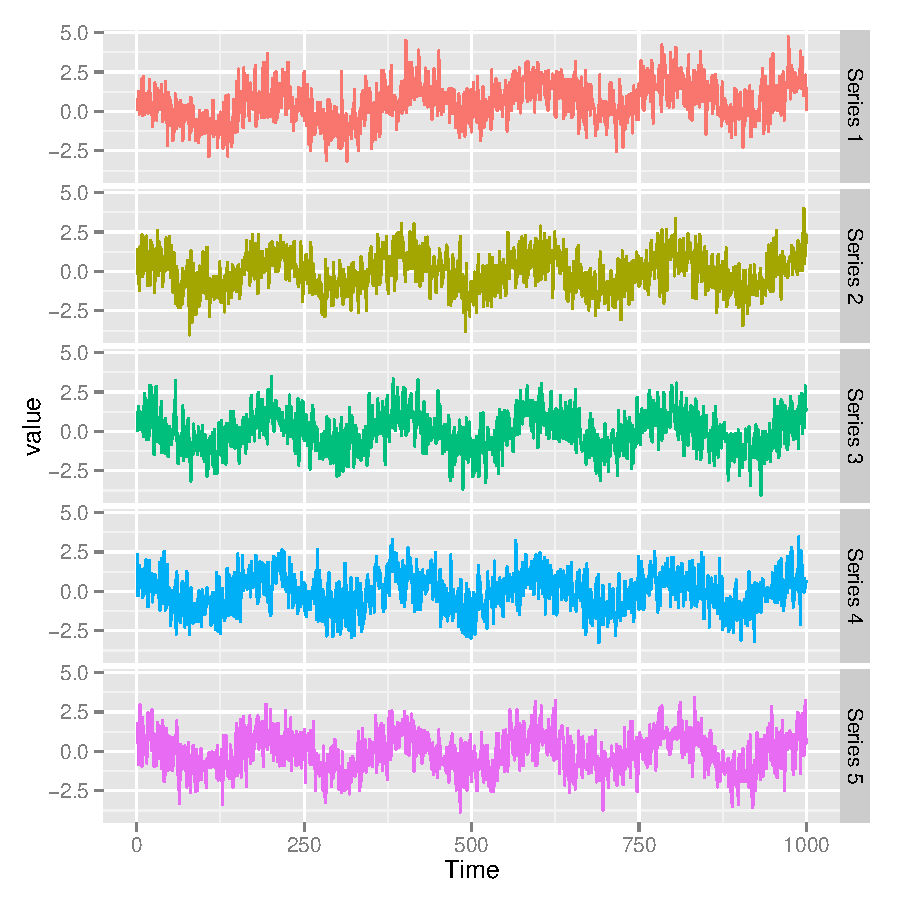
\includegraphics{pairwiseSNHT-005}

\begin{Schunk}
\begin{Sinput}
> dist<-matrix(0,5,5)
> #dist is a symmetric matrix
> upper<-matrix(c(rep(0,1),100,100,100,100, rep(0,2),200,141,141,
+               rep(0,3),141,141, rep(0,4),200, rep(0,5)), 
+               nrow=5,ncol=5)
> dist<-t(upper)+upper
> colnames(dist)<-rownames(dist)<-1:5
> dist
\end{Sinput}
\begin{Soutput}
    1   2   3   4   5
1   0 100 100 100 100
2 100   0 200 141 141
3 100 200   0 141 141
4 100 141 141   0 200
5 100 141 141 200   0
\end{Soutput}
\end{Schunk}

This is the distance matrix which is needed as an input parameter for pairwiseSNHT. It contains as (i,j)-th entry the distance between location i and j. It is therefore always a symmetric matrix with diagonal 0 and can be generated through the upper or lower diagonal matrix as done in the code.

\begin{Schunk}
\begin{Sinput}
> colnames(baseData)<-"1":"5"
> baseData <- data.frame(time=1:1000, baseData)
> baseData <- melt(baseData, id.vars = "time")
> baseData$variable <- gsub("X", "", baseData$variable)
> colnames(baseData) <- c("time", "location", "data")
> baseData <- baseData[, c("data", "location", "time")]
> out1 <- pairwiseSNHT(baseData, dist, k=3, period=12, crit=20, returnStat=T)
> pairs <- colnames(out1)
> pairs
\end{Sinput}
\begin{Soutput}
[1] "1-2" "1-3" "1-4" "1-5" "2-4" "2-5" "3-4" "3-5"
\end{Soutput}
\begin{Sinput}
> str(out1)
\end{Sinput}
\begin{Soutput}
 num [1:1000, 1:8] NA NA NA NA NA NA NA NA NA NA ...
 - attr(*, "dimnames")=List of 2
  ..$ : NULL
  ..$ : chr [1:8] "1-2" "1-3" "1-4" "1-5" ...
\end{Soutput}
\end{Schunk}

\textit{pairs} are the unique pairs which are formed by using $k=3$ neighbours.\\

Remark: If there are more than k neighbours with the same distance to a certain location, then more than k neighbours are considered. In this example, location 2,..4 all have the distance 100 to location 1 (see distance matrix), therefore all these 4 locations are paired with location 1. This means that all 4 difference series are used by pairwiseSNHT.\\

\textit{out1} is the matrix with the calculated SNHT statistic for each time point and each pair. Only NA's are displayed through \textit{str()} since period was chosen to be 12, i.e., for the first and last 12 values in each time series, there is not assigned any SNHT statistic. This is due to the definition of the SNHT statistic (see: \cite{haimberger07}).

Let us plot the obtained SNHT statistics for each pair.

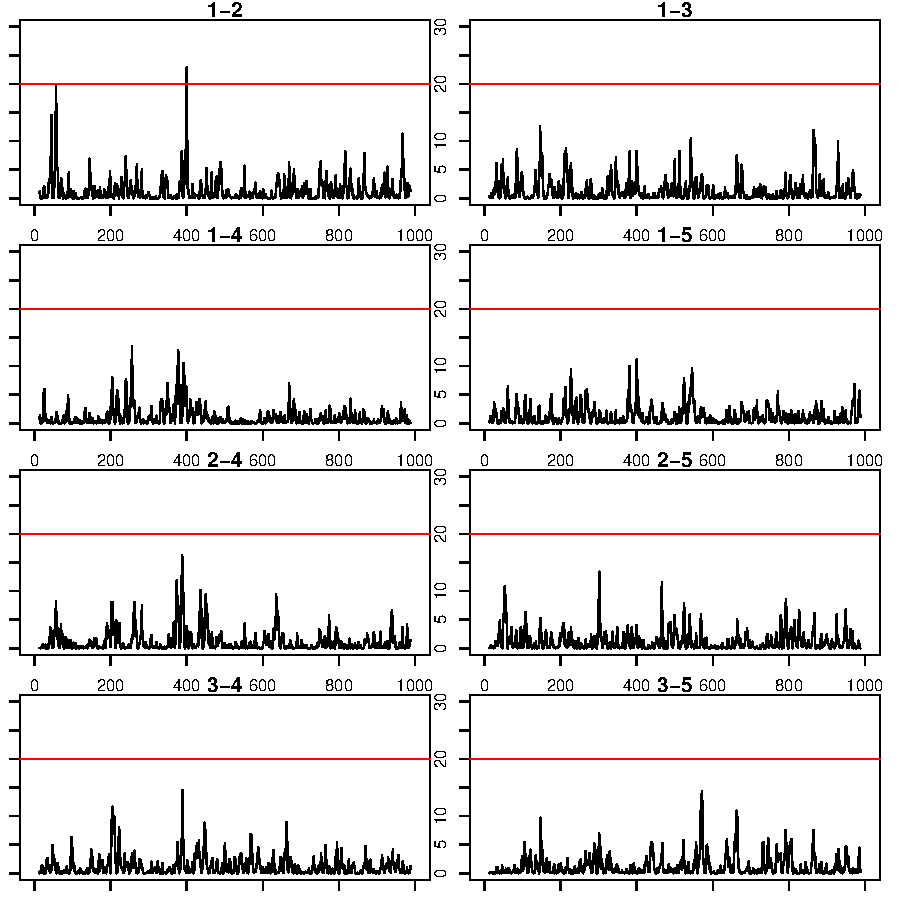
\includegraphics{pairwiseSNHT-008}

One can now clearly see that it is most likely that a changepoint occured at time 400. This changepoint as well as its magnitude is also obtained through setting returnStat=FALSE in pairwiseSNHT. Furthermore, the corrected data can be accessed through \textit{out2\$breaks} respectively \textit{out2\$data}.

\begin{Schunk}
\begin{Sinput}
> out2 <- pairwiseSNHT(baseData, dist, k=3, period=12, crit=20, returnStat=F)
> out2$breaks
\end{Sinput}
\begin{Soutput}
  time location shift
1    1        1     1
\end{Soutput}
\begin{Sinput}
> str(out2$data)
\end{Sinput}
\begin{Soutput}
'data.frame':	5000 obs. of  3 variables:
 $ data    : num  0.0376 0.7055 1.2544 -0.16 1.1835 ...
 $ location: Factor w/ 5 levels "1","2","3","4",..: 1 1 1 1 1 1 1 1 1 1 ...
 $ time    : int  1 2 3 4 5 6 7 8 9 10 ...
\end{Soutput}
\end{Schunk}

One can now check if the corrected data, which is stored in \textit{out2\$data} provides better results, i.e., the SNHT statistic does no longer exceed the critical value.

\begin{Schunk}
\begin{Sinput}
> newPair2 <- out2$data
> outNew1 <- pairwiseSNHT(newPair2,dist,k=3,period=12,crit=20,returnStat=T)
> par(mfrow=c(4,2),mar=c(1,1,1,1))
\end{Sinput}
\end{Schunk}
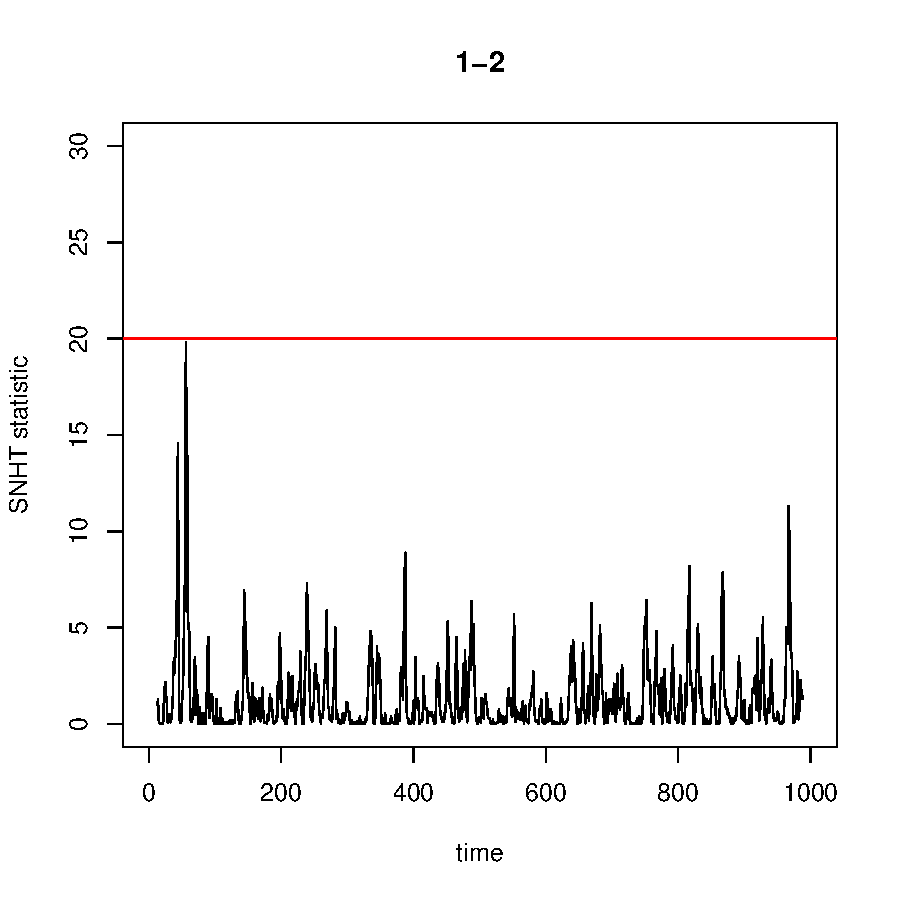
\includegraphics{pairwiseSNHT-011}


\bibliography{mybib}

\end{document}
